\subsection{
  Replies to comments received from Kate Scholberg - Jan. 06, 2013 }

\begin{enumerate}

%........................................................................................................
\vspace{5 mm}
\item
{\em
  ``p. 5-6 and Table 1  about normalization: 
  I assume the "events generated" are interactions the full ID, and "events in 
  fiducial volume" are triggered MC events (i.e. without any reduction cuts).  
  So the difference between the columns is mostly fiducial volume, right?  
  Please clarify briefly.''
}\\
\\
That is correct. 
Some additional clarifications are needed. 
The numbers of MC events in the fiducial volume (shown in the 4$^{th}$ column) are those for which the
{\em reconstructed} vertex lies within the fiducial volume.
In some of these MC events the true vertex may lie outside the fiducial volume, but this 
might also happen with actual data.
The events shown in that column are those used for constructing the MC templates described in the text.
However the true vertex position is used when calculating the absolute normalization for each sample,
using the quoted number of events per 22.5 kt fiducial per 10$^{21}$ POT.

%........................................................................................................
\vspace{5 mm}
\item
{\em
  ``p. 8-9 The text is a bit confusing about how reweighting was done ... 
  sounds as if first NA61 reweighting, then BANFF (on the same sample)... 
  please describe clearly.''
}\\
\\
That's correct. First, NA61 reweighting is applied to the nominal MC, i.e.\ 
the nominal 2011a Run 1+2+3 flux is reweighted to the 2011b\_v3.2 Run 1+2+3 flux.
Then BANFF reweighting is applied to the NA61-tuned MC, which involves reweighting the MC
to the BANFF best-fit values.
The starting point for the BANFF fit itself was an NA61-tuned MC, so the above 
2-step reweighting process is appropriate.	

%........................................................................................................
\vspace{5 mm}
\item
{\em
  ``p. 9  I know the answer is "it's negligibly small", 
  but please be quantitative about the amount of tau events expected.''
}\\
\\
Unfortunately, it is not easy to provide an exact numerical answer since, on the basis that 
the contribution is ``negligibly small'', no $\nu_{\tau}$ SK samples were generated.
However, an estimate is given below.

In Fig.\ \ref{fig:nutauccrate}, the black histogram shows the $\nu_\mu$-CC event rate
per 50 MeV bin per 22.5 kton of water fiducial mass and per $10^{21}$ POT, 
as predicted by the nominal MC 
before any single $\mu$-like ring reduction cuts.
Scaled to an exposure of 3.010 $\times 10^{21}$ POT, 
there are 314.8 events under this curve. 
This spectrum is reweighted using the following succession of steps in order 
to emulate the $\nu_{\tau}$-CC spectrum for events where a muon is present in the final state.
\begin{itemize}
\item
  Apply the $\nu_\tau$ appearance probability, P($\nu_\mu \rightarrow \nu_\tau$), 
  computed in a 3-flavour framework including matter effects in constant density matter.
  The following 23-sector oscillation parameters are used:
  $|\Delta m^{2}_{32}|$ = 2.44$\times$10$^{-3}$ $eV^{2}/c^{4}$ and $\sin^{2}2\theta_{23}$ = 1.0 (Run 1+2+3 best-fit values).
  2012 PDG values are used for $\sin^{2}2\theta_{13}$, $\sin^{2}2\theta_{12}$ and $\Delta m^{2}_{21}$ and $\delta_{CP}$=0. 
  The normal hierarchy is assumed. 
  This reweighted spectrum is shown in red.
\item
  Apply the ratio of the $\nu_\tau$ to $\nu_\mu$ 
  inclusive CC interaction cross-sections on water. 
  This reweighted spectrum is shown in blue.
\item
  Apply the branching ratio for $\tau \rightarrow \mu+X$,
  assuming that no other decay channel is likely to contaminate the single $\mu$-like ring sample.
  This reweighted spectrum is shown in magenta.
\end{itemize}

Scaled to an exposure of 3.010 $\times 10^{21}$ POT, there are 0.02 events under the spectrum shown in 
magenta. This number represents an upper limit on the contribution of $\nu_\tau$ CC events in the 
single $\mu$-like ring sample, since the single $\mu$-like ring cut efficiency is not included.
Assuming that the $\mu$-like ring cut efficiency for $\nu_\tau$ CC events, where the $\tau$-lepton decays
to a muon, is similar to the cut efficiency for $\nu_\mu$ CC events, then the expected 
contribution of $\nu_\tau$ CC events is $\sim$ 0.01 events.

\begin{figure*}[htb]
\center
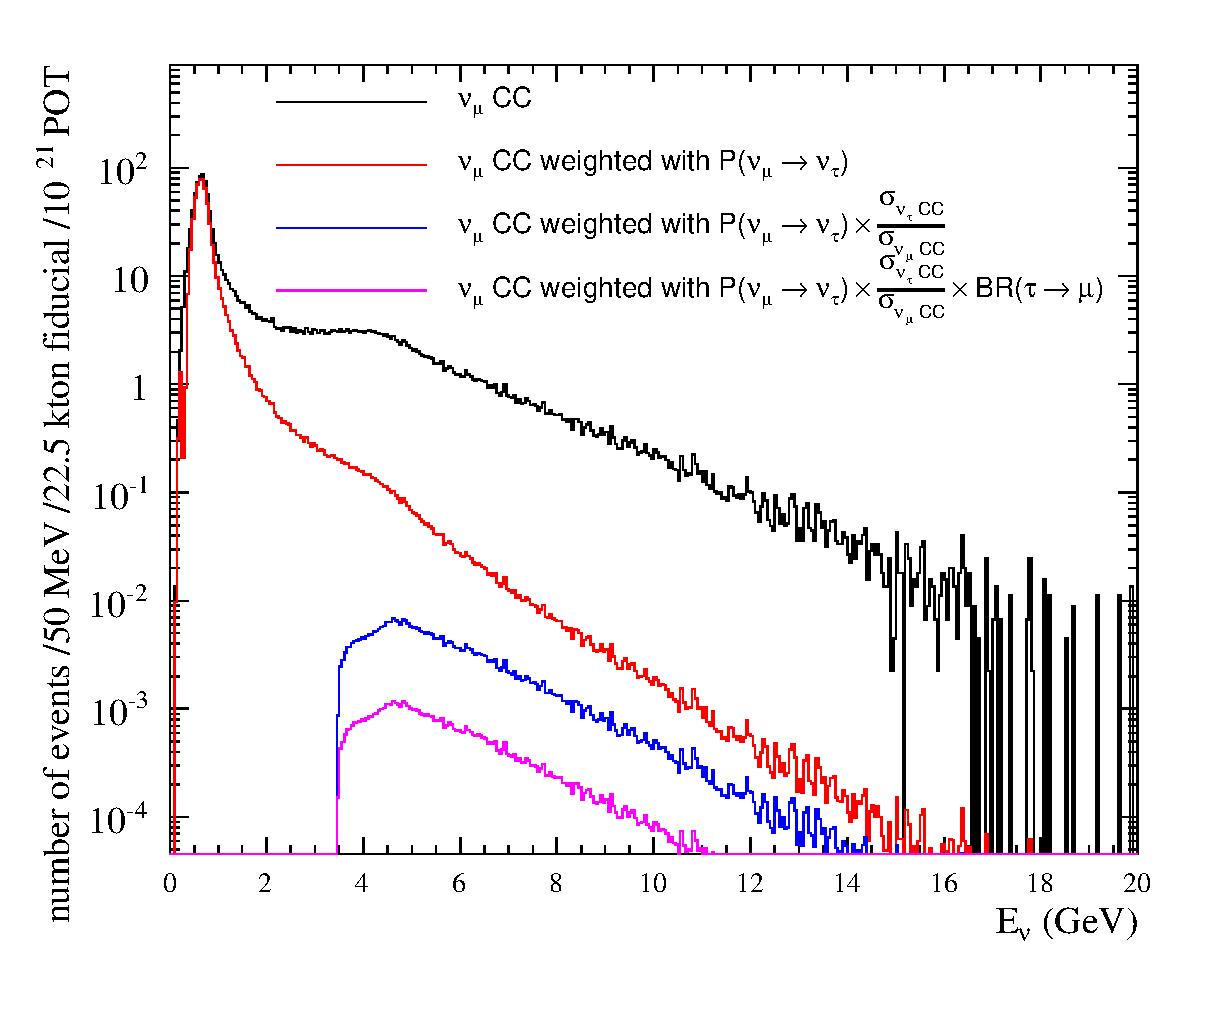
\includegraphics[width=35pc]{./images/nutau_spectrum_fidvol.eps}
\caption {
  Emulated event rate of $\nu_\tau$ CC events, where a muon is present in the final state 
  derived from the $\nu_\mu$ CC event rate (see text for details).
}
\label{fig:nutauccrate}
\end{figure*}



%........................................................................................................
\vspace{5 mm}
\item
{\em
  ``p. 11 Fig 6 and similar spectrum plots:  
  I would favor "Number of events per bin" on the y-axis (especially for outside consumption).''
}\\
\\
In version 2 of T2K-TN-141, the y-axis label of all similar plots will be modified
as suggested.

%........................................................................................................
\vspace{5 mm}
\item
{\em
  ``p. 28  "All of these choices are implemented in the VaLOR oscillation analysis"-- 
  not sure what this means-- that they can be selected as options for fitting?''
}\\
\\
Exactly. 
The VaLOR analysis code can switch transparently between different conventions.
For example, in our joint 3-flavour oscillation analysis 
we typically fit for $sin^{2}(\theta)$, rather than $sin^{2}(2\theta)$ 
\footnote{
See, http://www.t2k.org/meet/collab/201209/talks/satam/Joint\ Oscillation\ Analysis\ Report\ -\ VaLOR
}.

%........................................................................................................
\vspace{5 mm}
\item
{\em
  ``p. 30-31 Some confusion with the figure numbers--  looks like  Fig 259 is the same as Fig 23.  
  It would be good to refer to the figures in the main text rather than the appendix
  (not a content issue, just makes it hard to read).''
}\\
\\
In version 2 of T2K-TN-141, the latex referencing will be fixed.

%........................................................................................................

\end{enumerate}
